\chapter{磁力、ベクトルポテンシャル、作用原理}

\lectureoverview{静電気力はよく知られた保存力のパターンに当てはまるが、磁力は速度に依存する。これをラグランジュ力学の枠組みに収めるために、まず必要なベクトル解析を展開し、磁場が源を持たないという性質を用いてベクトルポテンシャルを導入し、そのゲージの自由度を調べ、その後で作用積分における磁気の項を構成する。}

\section{新しい種類の力}

角運動量、ジャイロスコープ、ポアソン括弧に関するこれまでの議論は、いくつかのテーマを結び合わせてきた。特に、磁場中の回転する帯電体は、ジャイロスコープとほぼ同じように歳差運動をする。ここでその類推から離れ、個々の荷電粒子の運動へと移る。

静電気力には新しい力学は必要ない。\(U(\mathbf x)\) をポテンシャルエネルギーとすれば、
\begin{equation}
  \mathbf F=-\nabla U(\mathbf x),
\end{equation}
となり、通常の議論から運動エネルギーとポテンシャルエネルギーの和が保存される。電荷 \(e\) の粒子が静電ポテンシャル \(V(\mathbf x)\) の中にあるとき、
\begin{equation}
  U(\mathbf x)=eV(\mathbf x),
  \qquad
  \mathbf F_{\mathrm{el}}=-e\nabla V.
\end{equation}
磁力は異なる形をとる。磁力は粒子の速度に依存するので、単にもう一つの通常のポテンシャルエネルギーを加えるだけでは導入できない。それにもかかわらず、磁力は作用原理から導かれ、ラグランジュ記述とハミルトン記述の両方を持つ。そこに到達するには、ベクトル解析における短いが本質的な挿入が必要である。

\section{場と局所的操作}

\subsection{場が記録するもの}

場は、空間の各点に、そして一般には各時刻に、物理量を割り当てる。温度と圧力はスカラー場である。風速はベクトル場である。電場と磁場はベクトル場である。他の理論には微視的なスケールでもスカラー場が含まれ、一方、重力はテンソル場によって記述される。ここでの議論では時間依存性を落とし、場を \(\mathbf x\) の関数として書く。

場の操作上の要点は局所性である。ある領域が袋の中に隠されていると想像しよう。その領域の電場を測定するには、そこに小さな試験電荷を置き、その加速度を観測する。力は電荷が位置する場所の場によって決まり、遠方の各源にいちいち問い合わせることで決まるのではない。同じことが磁場と運動する試験電荷についても成り立つ。後にベクトルポテンシャルはこの単純な描像に条件を付けることを強いるが、ここから始めるのが適切である。

\subsection{微分演算子}

微分は場を別の場に変える。3つの空間微分をまとめて
\begin{equation}
  \nabla
  =
  \left(
    \frac{\partial}{\partial x},
    \frac{\partial}{\partial y},
    \frac{\partial}{\partial z}
  \right).
\end{equation}
と書く。この記号は \emph{del} または \emph{nabla} と読む。逆さにした三角形の外観は記憶に残りやすいが、その本当の意義は、成分が微分演算子であるベクトルのように形式的に振る舞うことにある。

これは通常の3次元物理空間であり、位相空間でも多粒子配置空間でもない。さらに、\(\nabla\) は単独で存在できるベクトル場ではない。何かに作用しなければならない。\(T(\mathbf x)\) がスカラーの温度場であれば、
\begin{equation}
  \nabla T
  =
  \left(
    \frac{\partial T}{\partial x},
    \frac{\partial T}{\partial y},
    \frac{\partial T}{\partial z}
  \right)
\end{equation}
はその勾配であり、真のベクトル場である。

\begin{figure}[htbp]
\centering
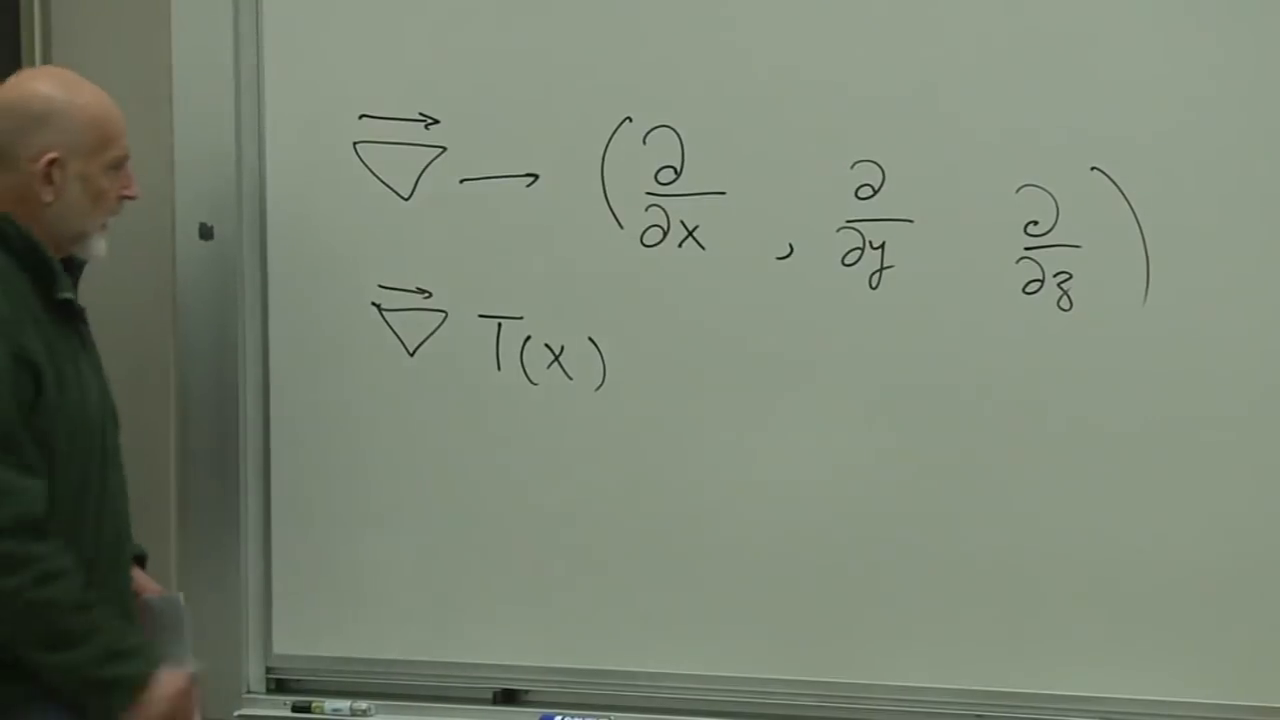
\includegraphics[width=0.82\textwidth]{lecture_09_figure_01.png}
\caption{黒板は \(\nabla\) を空間微分演算子のベクトルとして導入し、それをスカラー場 \(T(\mathbf x)\) に作用させ始める。}
\lectureframe{00:11:30}
\end{figure}

スカラーとは、単に1つの成分で書かれた量のことではない。その値が座標軸の向きに依存しない量のことである。温度が標準的な例である。ベクトル場 \(\mathbf E\) が与えられたとき、局所的な表式 \(\mathbf E\cdot\mathbf E\) もまたスカラーである。対照的に、場を積分してポテンシャルを構成することは非局所的な操作であり、経路に沿った値を用いる。

\subsection{発散}

ベクトル場 \(\mathbf A=(A_x,A_y,A_z)\) に対して、スカラー
\begin{equation}
  \nabla\cdot\mathbf A
  =
  \frac{\partial A_x}{\partial x}
  +\frac{\partial A_y}{\partial y}
  +\frac{\partial A_z}{\partial z}
\end{equation}
はその発散である。流体の言葉でいえば、正の発散は外へ流れ出そうとする局所的な傾向を表し、負の発散は内へ収束しようとする傾向を表す。流体の源は正の発散を生み、吸い込み口は負の発散を生む。この描像は定性的であるが、磁場が源を持たないという性質を明快にするであろう。

\section{外積、イプシロン記号、回転}

\subsection{成分による外積}

二つのベクトル\(\mathbf V\)と\(\mathbf A\)に対し、外積の一つの成分は
\begin{equation}
  (\mathbf V\times\mathbf A)_x
  =
  V_yA_z-V_zA_y.
\end{equation}
である。残りの二つは\(x\to y\to z\to x\)と巡回させることで得られる。\(x,y,z\)を添字\(1,2,3\)に置き換えると便利である。クロネッカーの記号は
\begin{equation}
  \delta_{ij}
  =
  \begin{cases}
    1,&i=j,\\
    0,&i\ne j,
  \end{cases}
\end{equation}
であり、レヴィ--チヴィタ記号は
\begin{equation}
  \epsilon_{123}=\epsilon_{231}=\epsilon_{312}=1,
  \qquad
  \epsilon_{132}=\epsilon_{321}=\epsilon_{213}=-1,
\end{equation}
によって定義され、任意の二つの添字が一致するときは常に\(\epsilon_{ijk}=0\)である。三時計回りの巡回順序が正符号を与え、向きを逆にすると負符号を与える。任意の一対の添字を入れ替えると符号が反転するので、\(\epsilon_{ijk}\)は完全反対称である。

また、総和規約も用いる。項の中で繰り返される添字は\(1\)から\(3\)まで和をとる。すると三つの外積の式は
\begin{equation}
  (\mathbf V\times\mathbf A)_i
  =
  \epsilon_{ijk}V_jA_k.
\end{equation}
となる。例えば\(i=1\)と置くと\((j,k)=(2,3)\)と\((3,2)\)だけが残り、
\begin{equation}
  (\mathbf V\times\mathbf A)_1
  =
  \epsilon_{123}V_2A_3
  +\epsilon_{132}V_3A_2
  =
  V_2A_3-V_3A_2.
\end{equation}
となる。したがって、この簡潔な記法はよく知られた成分の規則を正確に含んでいる。

\subsection{反対称行列に姿を変えたベクトル}

第二の表現がある：
\begin{equation}
  V_iA_j-V_jA_i
  =
  \epsilon_{ijk}(\mathbf V\times\mathbf A)_k.
\end{equation}
左辺は二つの添字をもち、\(i\leftrightarrow j\)の下で反対称である。行列として見ると
\begin{equation}
  M_{ij}
  =
  \begin{pmatrix}
    0&M_{12}&M_{13}\\
    -M_{12}&0&M_{23}\\
    -M_{13}&-M_{23}&0
  \end{pmatrix}.
\end{equation}
という形をしている。対角成分は消え、下三角部分は上三角部分によって定まる。したがって独立な成分は三つである。

\begin{figure}[htbp]
\centering
\includegraphics[width=0.82\textwidth]{lecture_09_figure_02.png}
\caption{外積の一成分と、その独立な成分を数えるために用いられる概略的な\(3\times3\)反対称配列。セル内の印は追加の記号ではなく記憶を助けるためのものである。}
\lectureframe{00:34:20}
\end{figure}

\begin{classroomqa}
\audiencequestion{外積、あるいは別のベクトルとの同一視は、三次元の外でも意味をもつだろうか。}
\lecturerresponse{反対称な二添字の対象は任意の次元で意味をもつが、それをベクトルと同一視することは三次元に特有である。三次元のベクトルは三つの成分をもち、反対称な\(3\times3\)行列は三つの独立な成分をもつ。四次元では対応する数は四と六である。なぜなら\(4(4-1)/2=6\)だからである。反対称な対象は依然として存在し、自然に二形式とみなされるが、それは別の四元ベクトルではない。}
\end{classroomqa}

\subsection{回転}

\(\mathbf V\)を\(\nabla\)に置き換えると回転が定義される：
\begin{equation}
  (\nabla\times\mathbf A)_i
  =
  \epsilon_{ijk}\frac{\partial A_k}{\partial x_j}.
\end{equation}
通常の成分では、
\begin{align}
  (\nabla\times\mathbf A)_x
  &=
  \frac{\partial A_z}{\partial y}
  -\frac{\partial A_y}{\partial z},\\
  (\nabla\times\mathbf A)_y
  &=
  \frac{\partial A_x}{\partial z}
  -\frac{\partial A_z}{\partial x},\\
  (\nabla\times\mathbf A)_z
  &=
  \frac{\partial A_y}{\partial x}
  -\frac{\partial A_x}{\partial y}.
\end{align}
である。発散が局所的な広がりを測るのに対し、回転は局所的な循環を測る。軸のまわりで回転する流体は、その軸に沿って非零の回転をもつ。この描像は速度場に対して特に鮮明であるが、定義は任意のベクトル場に当てはまる。

\section{二つの構造的恒等式}

二つの事実が数学的な作業のほとんどすべてを担う：
\begin{equation}
  \nabla\cdot(\nabla\times\mathbf A)=0,
  \qquad
  \nabla\times(\nabla s)=0.
\end{equation}
第一は、二階導関数が対称である一方で\(\epsilon_{ijk}\)が反対称であることから従う：
\begin{equation}
  \nabla\cdot(\nabla\times\mathbf A)
  =
  \epsilon_{ijk}\partial_i\partial_j A_k
  =0.
\end{equation}
第二は、混合偏導関数の等しさから従う：
\begin{equation}
  \bigl[\nabla\times(\nabla s)\bigr]_i
  =
  \epsilon_{ijk}\partial_j\partial_k s
  =0.
\end{equation}

\begin{figure}[htbp]
\centering
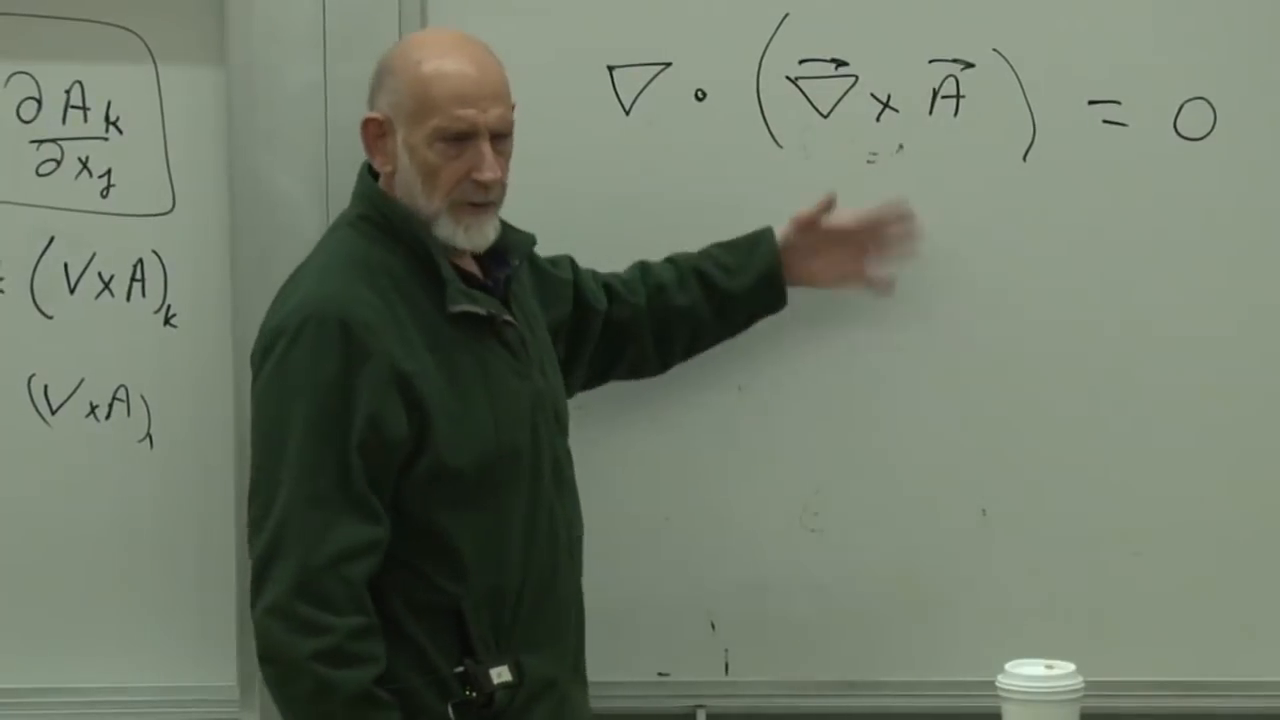
\includegraphics[width=0.80\textwidth]{lecture_09_figure_03.png}
\caption{黒板に書かれた第一の恒等式：あらゆる回転の発散は消える。}
\lectureframe{00:38:26}
\end{figure}

これらは易しい向きであり、講義が約束した宿題や抜き打ち試験に適している。逆の命題にはより多くの注意が必要である。局所的には、あるいは適切な単連結または可縮な領域上で大域的には、
\begin{align}
  \nabla\cdot\mathbf F=0
  &\quad\Longrightarrow\quad
  \mathbf F=\nabla\times\mathbf A,\\
  \nabla\times\mathbf F=0
  &\quad\Longrightarrow\quad
  \mathbf F=\nabla s.
\end{align}
である。領域についての条件がなければ、穴やその他の大域的な位相的性質がこれらの結論を妨げうる。講義では局所形を用いるが、それはまさに以下で必要とされるものである。

\section{なぜ磁場は回転なのか}

\subsection{観測される磁気源はない}

磁場\(\mathbf B\)は、荷電粒子や電流に対する効果を通じて操作的に定義される。磁気単極子のない通常の電磁気学では、
\begin{equation}
  \nabla\cdot\mathbf B=0.
\end{equation}
である。これは、発散が電荷密度に比例する電場とは異なる。電荷は電束の源と吸い込みである。磁束の孤立した源や吸い込みは観測されていない。

磁気単極子があればこの式は変わる。統一場理論はしばしばそのような対象の存在を期待する理論的な理由を与えるが、もし存在するとしても、利用可能な実験で生成するには質量が大きすぎるかもしれない。したがって現在の理論は磁荷密度を零として進む。

\begin{classroomqa}
\audiencequestion{磁気単極子とは何だろうか。普通の磁石にはすでに北極と南極がある。}
\lecturerresponse{孤立した単極子は、電荷に類似した、磁場の真の源または吸い込みであろう。普通の棒磁石は異なる。その北極付近から出る磁力線は空間を曲がって南極へ戻り、磁石の材料を通って続く。外部から源と吸い込みに見えるものは、隠れた管を通る流体のように、つながっている。磁束の正味の生成も消滅もない。}
\end{classroomqa}

\begin{figure}[htbp]
\centering
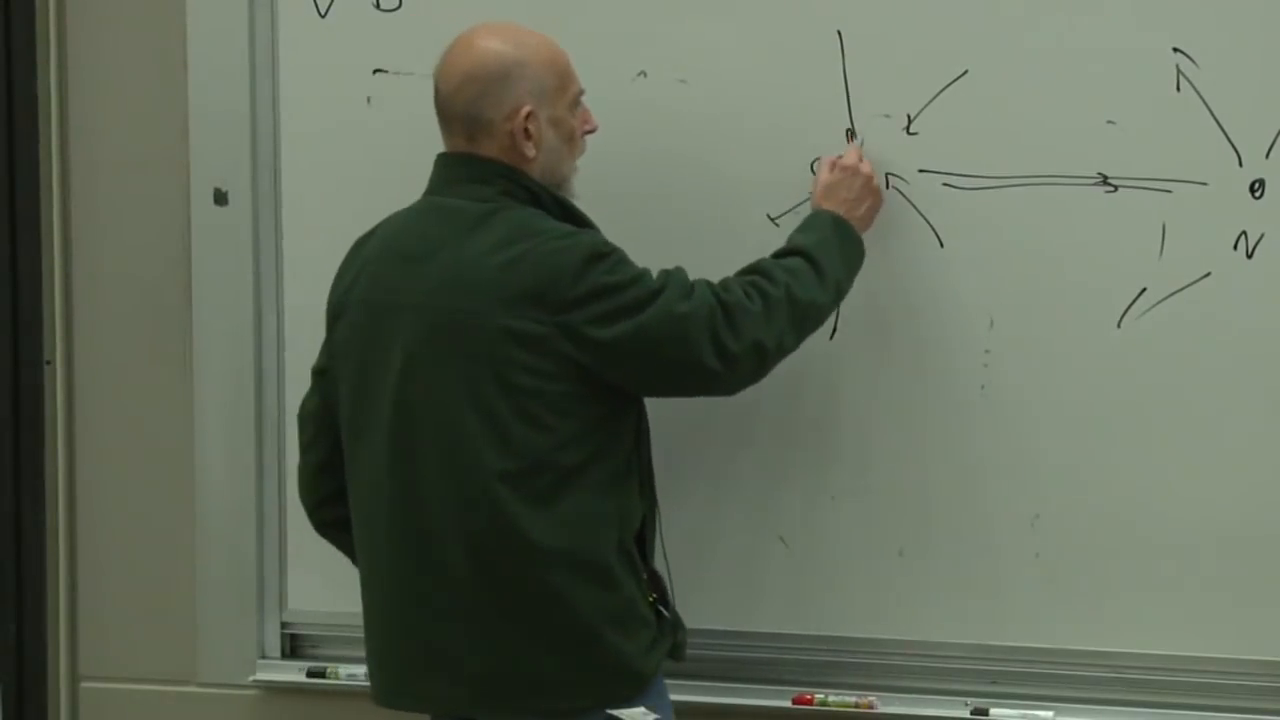
\includegraphics[width=0.76\textwidth]{lecture_09_figure_04.png}
\caption{黒板は、見かけの北と南の源を対比しつつ、それらの磁力線を磁石を通してつなぎ、磁束がそこで始まったり終わったりしないことを強調している。}
\lectureframe{00:44:56}
\end{figure}

\(\mathbf B\) は発散がないので、逆定理により、少なくとも局所的には
\begin{equation}
  \boxed{\mathbf B=\nabla\times\mathbf A}.
\end{equation}
と書ける。場 \(\mathbf A\) がベクトルポテンシャルである。一見すると、これは測定可能な場 \(\mathbf B\) を不必要に言い換えたものに見えるかもしれない。その目的は、作用を構成するときに初めて明らかになる。

\subsection{ベクトルポテンシャルは一意ではない}

\(\mathbf A\) が一つのベクトルポテンシャルならば、
\begin{equation}
  \mathbf A'=\mathbf A+\nabla s
\end{equation}
もまたベクトルポテンシャルである。なぜなら
\begin{equation}
  \nabla\times\mathbf A'
  =
  \nabla\times\mathbf A+\nabla\times(\nabla s)
  =
  \mathbf B.
\end{equation}
だからである。この置き換えは \emph{ゲージ変換} である。磁場はゲージ不変である。

\begin{figure}[htbp]
\centering
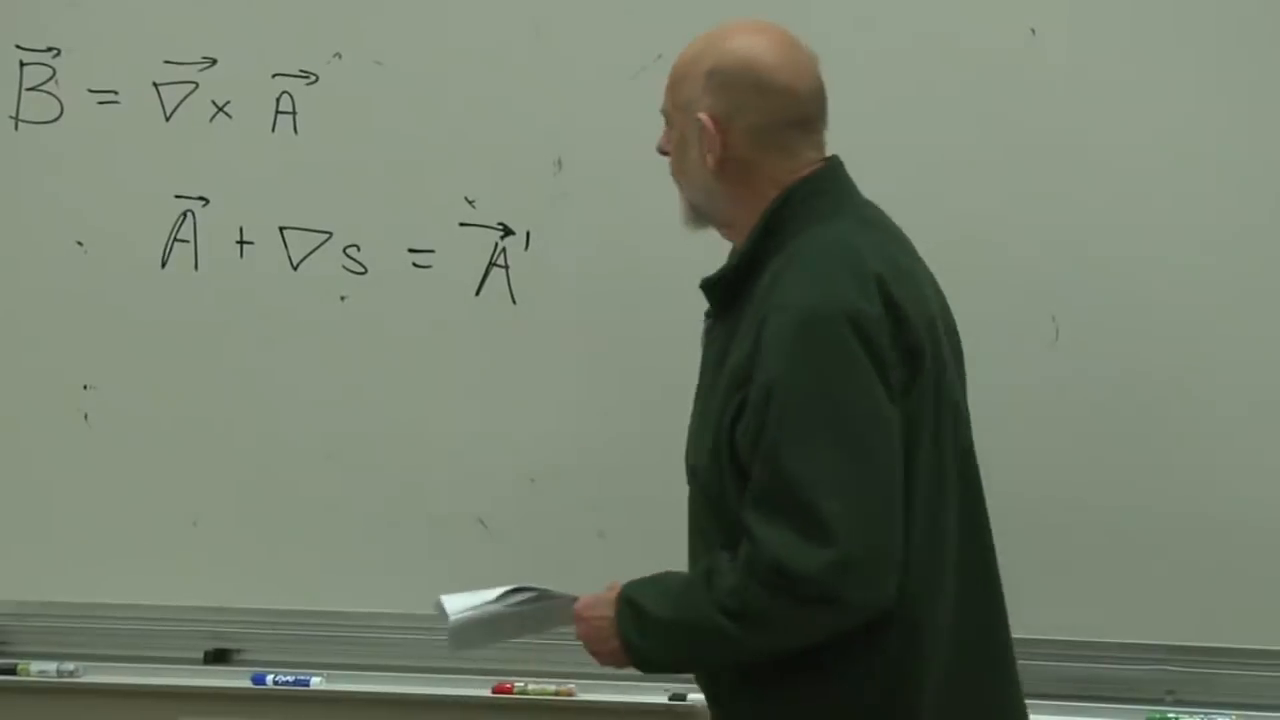
\includegraphics[width=0.80\textwidth]{lecture_09_figure_05.png}
\caption{定義関係 \(\mathbf B=\nabla\times\mathbf A\) とゲージのずれ \(\mathbf A'=\mathbf A+\nabla s\) が黒板に並んで現れている。}
\lectureframe{01:03:01}
\end{figure}

発音は \emph{ゲージ} であり、\emph{グアッシュ} でも \emph{ガウジ}-- でもない——講義はこの区別を半ば冗談めかした厳しさで徹底する。この語自体は歴史的なものである。異なる場所にある長さ標準の比較とこの自由度を結びつけようとした初期の試みから生じた。その元々の解釈は生き残らなかったが、名前は残った。

\begin{classroomqa}
\audiencequestion{この議論で、ゲージ変換とは具体的に \(\mathbf A\mapsto\mathbf A+\nabla s\) を意味するのですか。}
\lecturerresponse{はい。それがここで用いられている完全な電磁気的変換である。Yang--Mills理論や他の場の理論におけるゲージ変換は同じ考えを一般化したものだが、電磁気学ではスカラーの勾配を加えるだけで十分である。}
\end{classroomqa}

この非一意性は、何が直接測定可能かを明らかにする。小さな領域内の荷電粒子は局所的な \(\mathbf B\) に応答し、ゲージ変換で関係づけられるすべてのベクトルポテンシャルはそこで同じ力を予言する。この古典的な種類の局所実験で \(\mathbf A\) に一意な値を割り当てるものは存在しない。

\begin{classroomqa}
\audiencequestion{勾配を加えることが非一意性の完全な記述ですか。}
\lecturerresponse{単純な領域上の局所的には、はい。もし \(\nabla\times\mathbf A'=\nabla\times\mathbf A\) ならば \(\nabla\times(\mathbf A'-\mathbf A)=0\) なので、差は勾配である。大域的には、多重連結な領域は追加の微妙さを持ちうる。定数ベクトルを加えることはすでに含まれている。定数ベクトルは線形なスカラー関数の勾配だからである。\(s\) 自体に定数を加えても、その勾配が消えるので何も変わらない。}
\end{classroomqa}

\begin{classroomqa}
\audiencequestion{ゲージ自由度に根底となる物理的理由があるなら、それは何ですか。}
\lecturerresponse{講義はそのより深い解釈を先延ばしにする。有用な第一歩は、この自由度を扱い、それが作用にどのように入るかを見ることである。形式に慣れれば、ゲージ記述が不可欠である理由を認識しやすくなる。}
\end{classroomqa}

\section{一つの磁場、多くのポテンシャル}

最も単純な例を考えよう。
\begin{equation}
  \mathbf B=b\,\hat{\mathbf z},
  \qquad
  B_x=B_y=0,
  \qquad
  B_z=b,
\end{equation}
ここで \(b\) は定数である。一つのベクトルポテンシャルは
\begin{equation}
  \mathbf A^{(1)}=(0,bx,0).
\end{equation}
である。実際、
\begin{equation}
  (\nabla\times\mathbf A^{(1)})_z
  =
  \frac{\partial A_y^{(1)}}{\partial x}
  -\frac{\partial A_x^{(1)}}{\partial y}
  =b,
\end{equation}
であり、他の回転成分は消える。

この選択は、物理的な場が \(x\)-\(y\) 面内で回転対称であるにもかかわらず、\(y\) 方向を特別扱いしているように見える。第二の選択は任意性を明示する。
\begin{equation}
  \mathbf A^{(2)}=(-by,0,0).
\end{equation}
これは
\begin{equation}
  (\nabla\times\mathbf A^{(2)})_z
  =
  0-\frac{\partial(-by)}{\partial y}
  =b.
\end{equation}
を与える。二つのポテンシャルの差は
\begin{equation}
  \mathbf A^{(2)}-\mathbf A^{(1)}
  =
  (-by,-bx,0)
  =
  \nabla(-bxy).
\end{equation}
である。したがってそれらはゲージ同値である。回転対称な選択
\begin{equation}
  \mathbf A^{(\mathrm{sym})}
  =
  \frac12\,\mathbf B\times\mathbf r
  =
  \left(-\frac{by}{2},\frac{bx}{2},0\right),
\end{equation}
も同じ族の別の要素である。

\begin{figure}[htbp]
\centering
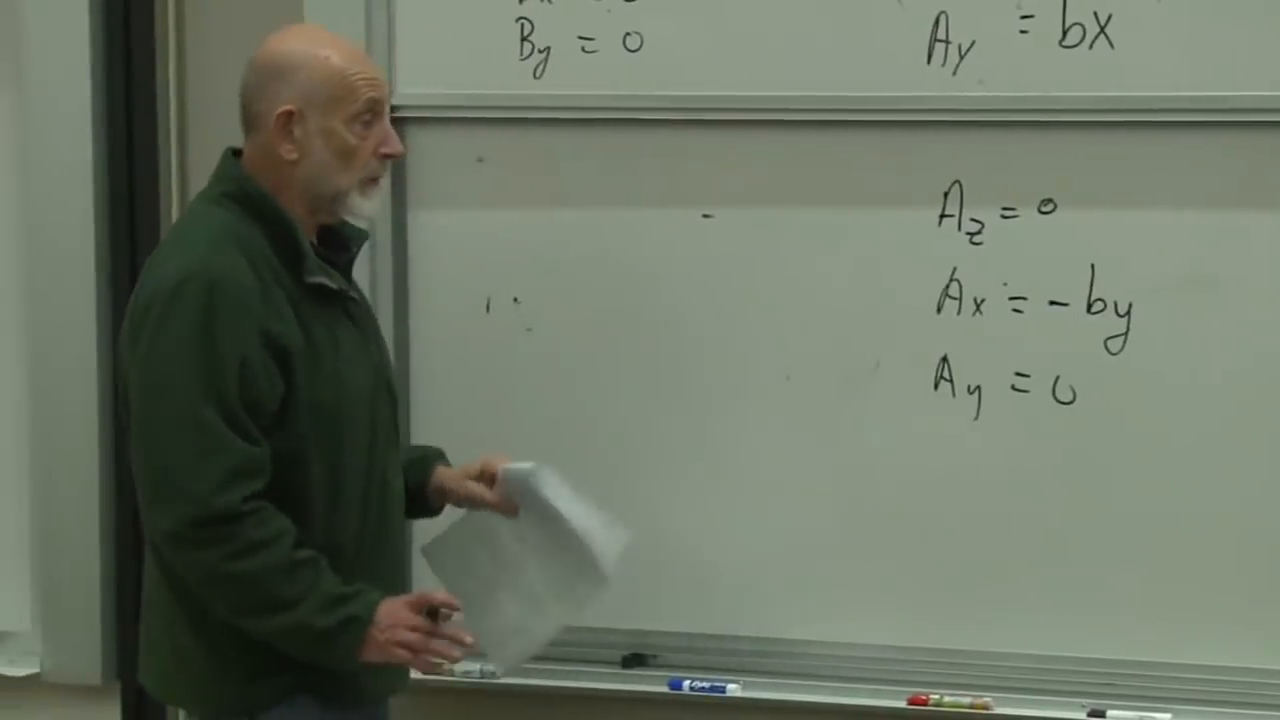
\includegraphics[width=0.80\textwidth]{lecture_09_figure_06.png}
\caption{黒板の二つのパネルには選択 \(A_y=bx\) と \(A_x=-by\) が示され、どちらも同じ一様な場 \(B_z=b\) を生じる。}
\lectureframe{01:07:20}
\end{figure}

\begin{classroomqa}
\audiencequestion{これは、場を生じるために電流を流すコイルを異なる配置にするという曖昧さと同じですか。}
\lecturerresponse{いいえ。電流の異なる配置は異なる物理的源であり、一つの領域で一致しても、他の場所では異なる場を生じうる。ゲージ自由度は磁場が至る所で指定された後にも残る。同じ物理的な \(\mathbf B\) は依然として多くのベクトルポテンシャルを持つ。}
\end{classroomqa}

\begin{classroomqa}
\audiencequestion{勾配を加えることを、ねじれを加えずに伸縮させることとして描けますか。}
\lecturerresponse{それは有用な幾何学的直観である。回転は局所的なねじれの部分を検出し、純粋な勾配は回転がゼロである。この主張は \(\nabla\times\nabla s=0\) に正確に表されている。}
\end{classroomqa}

\begin{classroomqa}
\audiencequestion{\(\mathbf A\)の向きと\(\mathbf B\)の向きの間には固定した関係があるか。}
\lecturerresponse{ゲージに依存しない関係は存在しない。上の例ではたまたま\(A_z=0\)となっているが、定数\(A_z\)を加えてもいかなる導関数も変わらない。そのとき\(\mathbf A\)はもはや\(\mathbf B\)に垂直ではなくなる。この古典的な議論において不変な物理的内容を持つのは回転のみである。}
\end{classroomqa}

静電学にもっと穏やかな類似物がある。\(\mathbf E=-\nabla V\)であるから、\(V\)を\(V+C\)に置き換えても\(\mathbf E\)は変わらない。\emph{ベクトルポテンシャル}という語は、通常のスカラーポテンシャルにおけるこの自由度との類推によって部分的に選ばれた。すなわち、物理的な場を変えないようにポテンシャルを変えることができるのである。

\section{ローレンツ力}

作用原理が再現しなければならない力の法則をここで述べることができる。ここで用いる規約では、
\begin{equation}
  \boxed{
  \mathbf F
  =
  e\left(
    \mathbf E+\frac{\mathbf v}{c}\times\mathbf B
  \right)
  =
  -e\nabla V+\frac{e}{c}\mathbf v\times\mathbf B
  }.
\end{equation}
記号\(e\)は粒子の電荷、\(\mathbf v=\dot{\mathbf x}\)はその速度、\(V\)はスカラーポテンシャルである。この記法に誘惑されて\(V\)と\(\mathbf v\)を混同してはならない。SIの言葉では\(V\)はボルトで、\(e\)はクーロンで測られる。表示された\(1/c\)はこの講義で用いる単位規約に属する。構造上の要点は単位に依存しない。

\begin{figure}[htbp]
\centering
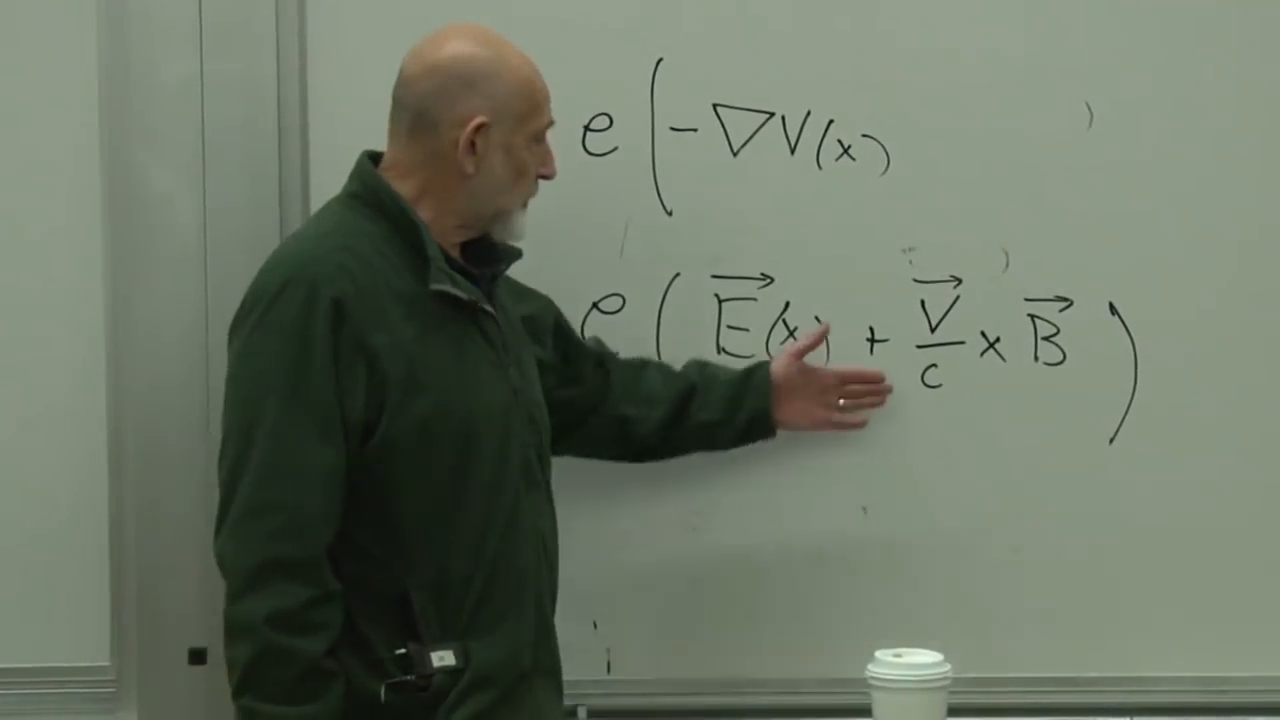
\includegraphics[width=0.82\textwidth]{lecture_09_figure_07.png}
\caption{ローレンツ力の電気項と磁気項がともに表示されている。磁気的な寄与は\(\mathbf v\times\mathbf B\)に比例する。}
\lectureframe{00:58:54}
\end{figure}

電気項は保存的であり、すでになじみ深い。磁気項は新しい。静止した粒子に対しては消え、\(\mathbf v\)と\(\mathbf B\)の両方に垂直である。したがって、
\begin{equation}
  \mathbf v\cdot\mathbf F_{\mathrm{mag}}
  =
  \frac{e}{c}\mathbf v\cdot(\mathbf v\times\mathbf B)
  =0.
\end{equation}
静磁場は軌道を曲げるが、粒子に対して仕事をしない。これは速度と逆向きで運動エネルギーを奪う粘性抵抗とは異なる。

因子\(v/c\)はまた、これらの規約で同程度の場のスケールに対して、ゆっくり動く粒子では磁気的効果が電気的効果よりしばしば小さい理由を示している。電子は十分軽いので大きな速度に達し、したがって磁気的偏向は依然として観測しやすい。

歴史的には、電流を運ぶ導線に働く力は、個々の電荷に働く力が分離されるより前に知られていた。ローレンツは、導線に働く力を各々の運動する電荷に速度依存項を割り当てることで理解できると認識した。電気と磁気を合わせた完全な表式は現在ローレンツ力の法則と呼ばれているが、本議論で新しい部分は磁気の項である。

\begin{classroomqa}
\audiencequestion{表式全体に別の記号があるのか、それとも磁気の部分だけがローレンツ力なのか。}
\lecturerresponse{表式全体は単に力\(\mathbf F=m\mathbf a\)であり、一般にローレンツ力と呼ばれる。磁気の項は歴史的にローレンツに最も直接結びつけられた部分である。電場と磁場は相対性理論によって深く関係しているが、その統一は現在の力学の問題には必要ない。}
\end{classroomqa}

\subsection{コリオリとの類推}

速度と固定ベクトルの外積は以前にも見た。角速度\(\boldsymbol\omega\)で回転する座標系では、コリオリ力は
\begin{equation}
  \mathbf F_{\mathrm{Cor}}
  =
  2m\,\mathbf v\times\boldsymbol\omega.
\end{equation}
と書ける。これは磁気力と同じ代数的形を持つ：
\begin{equation}
  2m\boldsymbol\omega
  \quad\longleftrightarrow\quad
  \frac{e}{c}\mathbf B.
\end{equation}
したがって、平面に垂直な一様磁場は、回転座標系が運動する物体を偏向させるのとほぼ同じように、荷電粒子の軌道を曲げる。

\begin{figure}[htbp]
\centering
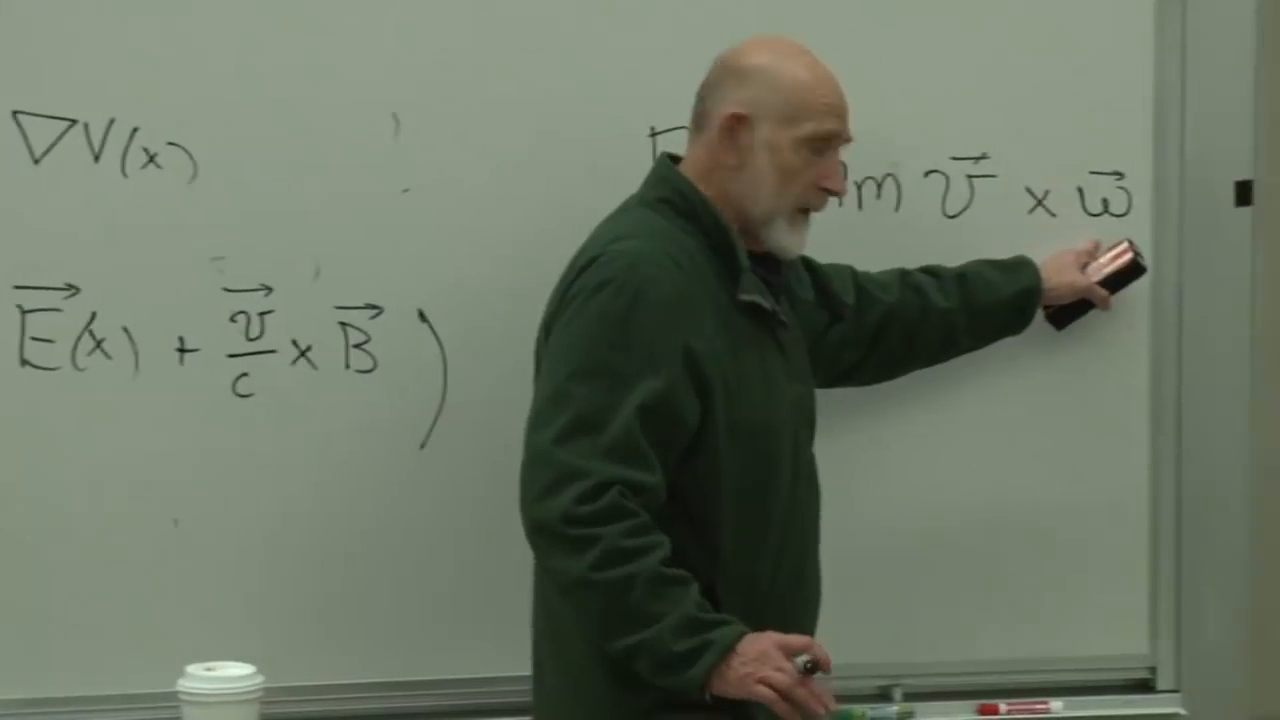
\includegraphics[width=0.82\textwidth]{lecture_09_figure_08.png}
\caption{ローレンツ力は左辺に残り、黒板は対応するコリオリの形\(2m\,\mathbf v\times\boldsymbol\omega\)を加える。}
\lectureframe{01:02:08}
\end{figure}

\begin{classroomqa}
\audiencequestion{コリオリ力は見かけの力と呼ばれる。速度に依存するから磁気力より実在性が低いのか。}
\lecturerresponse{速度依存性は問題ではない。回転台上の人は運動する物体を保持し、コリオリ力を感じることができる。それが見かけの力と呼ばれるのは、慣性系では消えるからであり、回転座標系はまさにそのような慣性項の存在によって定義される。\emph{実在}という語は、どの座標系でどの方程式を用いているかを述べるよりも有用でないことが多い。}
\end{classroomqa}

この類推は小さな思考実験にまで押し進められる。回転台上では、適切な静電場が選んだ粒子について遠心力の項を打ち消すことができ、適切な一様磁場がコリオリの項を打ち消すことができる。打ち消しは選んだ電荷対質量比に対してのみ働く。電気力と磁気力は\(e\)に比例してスケールするのに対し、慣性力は\(m\)に比例してスケールするからである。電子に合わせた場の配置は、異なる\(e/m\)を持つ粒子に対して同じ項を打ち消さないであろう。

\section{荷電粒子の作用の構成}

\subsection{端点を固定した停留作用}

ここで中心的な問いを立てよう。ローレンツ力を作用原理から導けるだろうか。答えはイエスであるが、ベクトルポテンシャルが不可欠である。粒子と\(\mathbf B\)のみから局所的に作ったラグランジアンは、必要な磁気力を生み出さない。この否定的な主張を証明する代わりに、成功する作用を直接構成する。

軌道\(\mathbf x(t)\)に対して、
\begin{equation}
  S[\mathbf x]
  =
  \int_{t_i}^{t_f}L(\mathbf x,\dot{\mathbf x},t)\,dt.
\end{equation}
と書く。講義では作用とベクトルポテンシャルに同じ手書きの文字を用いているが、ここでは作用に\(S\)、ベクトルポテンシャルに\(\mathbf A\)を用いる。物理的な経路は、両端点を固定した変分の下で\(S\)を停留させる。伝統的な\emph{最小作用}という言い回しは便利であるが、極値は最小である必要はないので、停留作用の方がより正確である。

端点を固定することは重要である。経路の両端を板に釘で留め、内部を揺らすと想像してもよい。これは通常の力学における軌道であり、弦理論の対象ではない。弦のイメージは変分を視覚化するための手段にすぎない。

\subsection{ラグランジアンに何が入りうるか}

すべての場を切ると、ラグランジアンは運動エネルギーである。
\begin{equation}
  L_0=\frac{m}{2}\dot{\mathbf x}^{\,2}.
\end{equation}
静電項もまた標準的である。
\begin{equation}
  L_{\mathrm{el}}=-eV(\mathbf x).
\end{equation}
磁気項はいくつかの手がかりを満たさなければならない。
\begin{enumerate}
  \item 電荷\(e\)に比例しなければならない。
  \item 講義の単位では因子\(1/c\)を含まなければならない。
  \item 速度を含まなければならない。
  \item 回転スカラーでなければならない。
\end{enumerate}

誘惑的な試み\(\mathbf B\cdot\dot{\mathbf x}\)はスカラーであり速度を含むが、誤った運動方程式を与える。正しい項はベクトルポテンシャルを用いる。
\begin{equation}
  L_{\mathrm{mag}}
  =
  \frac{e}{c}\mathbf A(\mathbf x)\cdot\dot{\mathbf x}
  =
  \frac{e}{c}A_i(\mathbf x)\dot x_i.
\end{equation}
したがって、時間に依存しない完全な電磁ラグランジアンは
\begin{equation}
  \boxed{
  L
  =
  \frac{m}{2}\dot{\mathbf x}^{\,2}
  +\frac{e}{c}\mathbf A(\mathbf x)\cdot\dot{\mathbf x}
  -eV(\mathbf x)
  }.
\end{equation}
である。講義10ではオイラー--ラグランジュ方程式を適用し、この表式がローレンツ力を生み出すことを明示的に示す。

\begin{figure}[htbp]
\centering
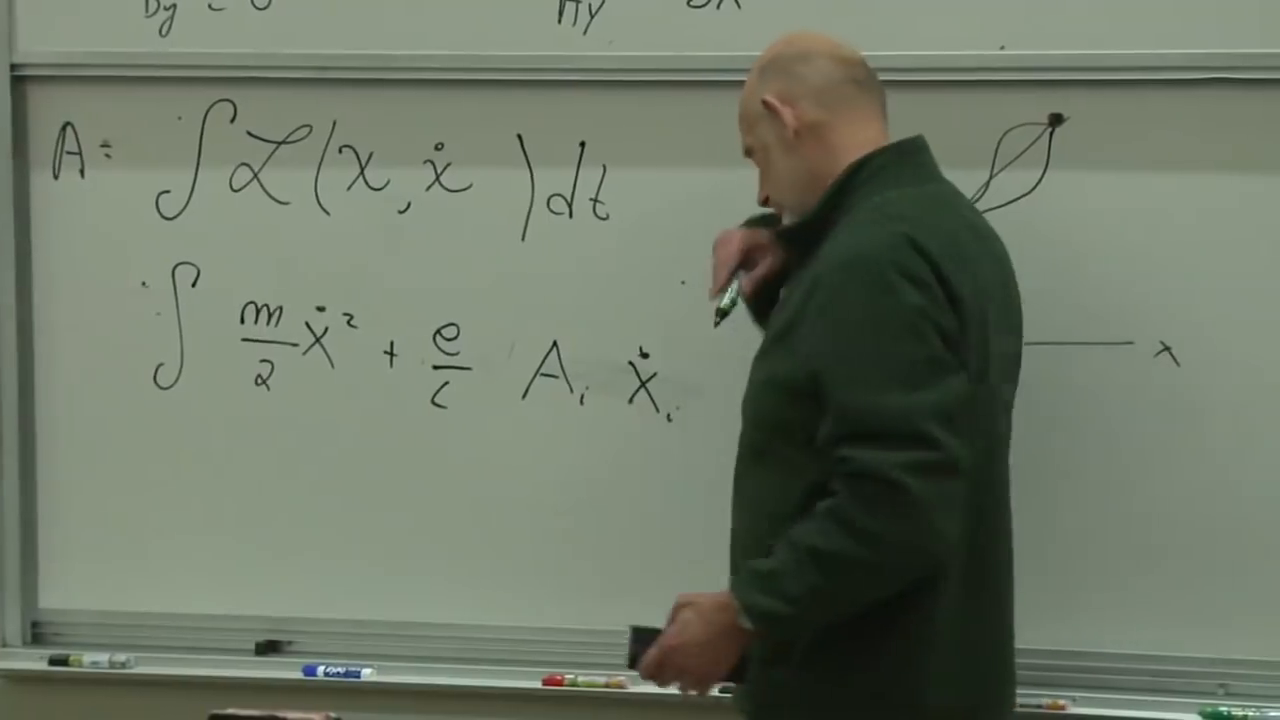
\includegraphics[width=0.82\textwidth]{lecture_09_figure_09.png}
\caption{作用の板書構成の完成形：自由な運動項と\((e/c)A_i\dot x_i\)。}
\lectureframe{01:26:36}
\end{figure}

\section{ゲージ変換は端点のみを変える}

作用への磁気的寄与は
\begin{equation}
  S_{\mathrm{mag}}
  =
  \frac{e}{c}
  \int_{t_i}^{t_f}A_i(\mathbf x)\dot x_i\,dt.
\end{equation}
である。\(\dot x_i\,dt=dx_i\)なので、これは粒子の経路\(\gamma\)に沿った線積分である。
\begin{equation}
  S_{\mathrm{mag}}
  =
  \frac{e}{c}\int_\gamma A_i\,dx_i
  =
  \frac{e}{c}\int_\gamma\mathbf A\cdot d\mathbf x.
\end{equation}
経路を短い線分に分割し、各線分に沿った\(\mathbf A\)の成分を取り、線分の長さを掛けて足し合わせる。これがこの積分の幾何学的な意味である。

次にゲージ変換
\begin{equation}
  A_i\longmapsto A_i+\partial_i s.
\end{equation}
を行う。作用は
\begin{align}
  \Delta S
  &=
  \frac{e}{c}\int_\gamma \partial_i s\,dx_i\\
  &=
  \frac{e}{c}\int_\gamma ds\\
  &=
  \frac{e}{c}
  \left[
    s(\mathbf x_f)-s(\mathbf x_i)
  \right].
\end{align}
だけ変化する。各無限小線分は、一方の端における\(s\)の値から他方の端における値を引いたものを寄与する。和を取ると、内部の寄与はすべて望遠鏡式的に相殺し、二つの端点だけが残る。

\begin{figure}[htbp]
\centering
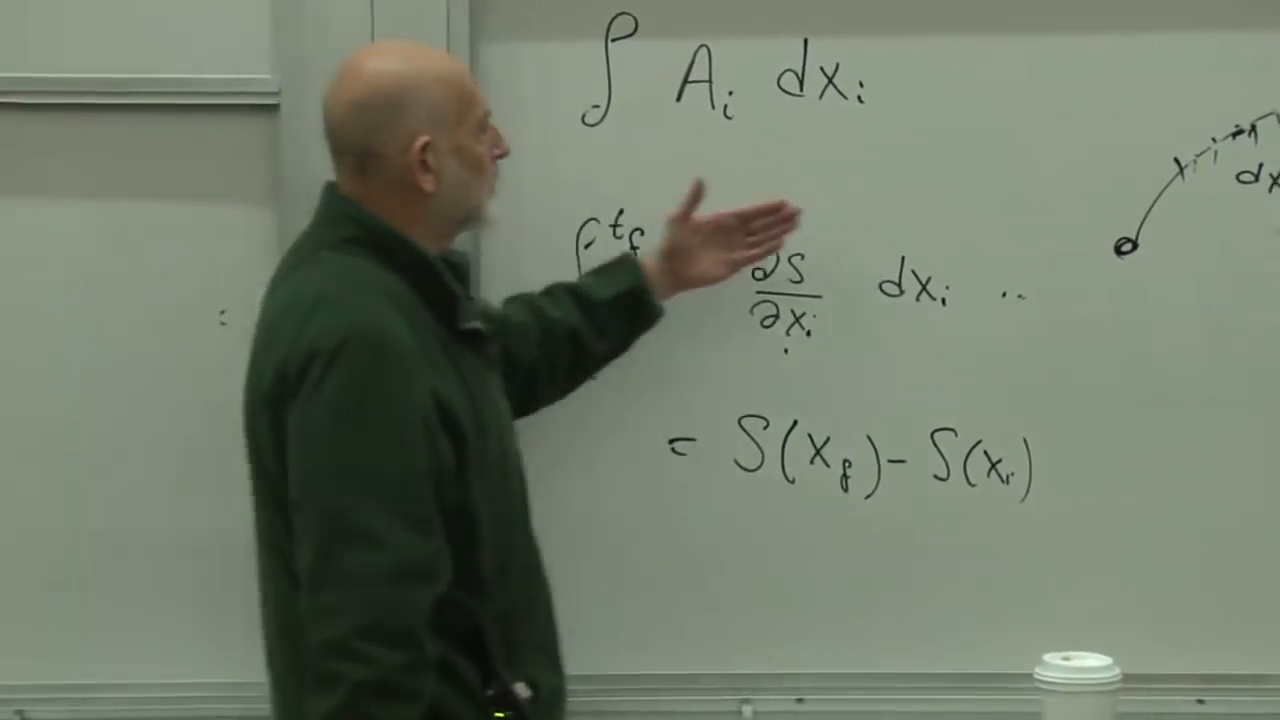
\includegraphics[width=0.82\textwidth]{lecture_09_figure_10.png}
\caption{線積分、その小さな経路線分への分割、および端点の結果\(s(\mathbf x_f)-s(\mathbf x_i)\)。}
\lectureframe{01:32:31}
\end{figure}

\begin{classroomqa}
\audiencequestion{ゲージ変換の下で作用が変化するなら、なぜ軌道は変化しないのか。}
\lecturerresponse{作用原理は初期点と終点を固定した経路を比較する。加えられた量はそれらの端点のみに依存するので、比較におけるすべての経路で同じ値をもつ。その変分はゼロである。数値としての作用は厳密には不変ではないが、オイラー--ラグランジュ方程式と物理的な軌道はゲージ不変である。}
\end{classroomqa}

この区別が講義の主要な概念的結果である。
\begin{equation}
  \begin{aligned}
    S&\ \hbox{may shift by an endpoint term},\\
    \delta S&\ \hbox{and the equations of motion do not}.
  \end{aligned}
\end{equation}
したがってゲージの自由度は作用原理と両立する。磁場によって一意な\(\mathbf A\)が選ばれなくても、ベクトルポテンシャルはラグランジアンに入りうる。

\section{議論の続き}

本講義は道具立てと作用を組み立てたが、その作用を変分する前で意図的に止まっている。次の段階はすでに定まっている。
\begin{enumerate}
  \item オイラー--ラグランジュ方程式を適用して
  \(\mathbf F_{\mathrm{mag}}=(e/c)\mathbf v\times\mathbf B\)を再現する。
  \item 正準運動量を計算する。これは\(m\mathbf v\)とは異なるであろう。
  \item ハミルトニアンを構成する。
  \item 保存則を同定する。
  \item 一様磁場中の荷電粒子の運動を解く。
\end{enumerate}

これらの結果への道筋は、なぜベクトルポテンシャルを導入したかを説明する。磁場は局所的に測定可能な回転であるが、ベクトルポテンシャルは粒子の経路と自然に結合する対象である。ゲージ変換はその結合を固定された端点においてのみ変え、力学を変えない。